

\tikzset{every picture/.style={line width=0.75pt}} %set default line width to 0.75pt        

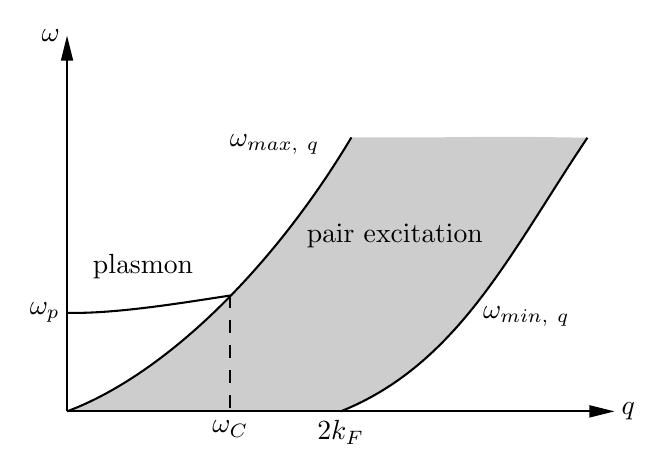
\begin{tikzpicture}[x=0.75pt,y=0.75pt,yscale=-1,xscale=1]
%uncomment if require: \path (0,300); %set diagram left start at 0, and has height of 300

%Shape: Polygon Curved [id:ds09427056966945702] 
\draw  [draw opacity=0][fill={rgb, 255:red, 155; green, 155; blue, 155 }  ,fill opacity=0.5 ] (122,251) .. controls (186.71,226.17) and (235.71,156.17) .. (259,119) .. controls (329.71,119.17) and (315.71,118.17) .. (372.71,119.17) .. controls (345.71,156.17) and (313.75,229.58) .. (253.85,251) .. controls (190.71,251.17) and (178.71,251.17) .. (122,251) -- cycle ;
%Straight Lines [id:da6805586288483829] 
\draw    (122,251) -- (383.71,251) ;
\draw [shift={(385.71,251)}, rotate = 180] [fill={rgb, 255:red, 0; green, 0; blue, 0 }  ][line width=0.08]  [draw opacity=0] (12,-3) -- (0,0) -- (12,3) -- cycle    ;
%Straight Lines [id:da22242400370456594] 
\draw    (122,251) -- (122,72) ;
\draw [shift={(122,70)}, rotate = 450] [fill={rgb, 255:red, 0; green, 0; blue, 0 }  ][line width=0.08]  [draw opacity=0] (12,-3) -- (0,0) -- (12,3) -- cycle    ;
%Curve Lines [id:da0536739950403895] 
\draw    (122,203.5) .. controls (145.71,204.17) and (180.71,198.17) .. (200.71,195.17) ;
%Curve Lines [id:da10994053272572524] 
\draw    (122,251) .. controls (170,233) and (222,181) .. (259,119) ;
%Curve Lines [id:da06610269106419042] 
\draw    (253.85,251) .. controls (310.71,228.17) and (335.71,174.17) .. (372.71,119.17) ;
%Straight Lines [id:da5827300524167289] 
\draw  [dash pattern={on 4.5pt off 4.5pt}]  (200.71,195.17) -- (200.71,251.17) ;

% Text Node
\draw (120,70) node [anchor=east] [inner sep=0.75pt]    {$\omega $};
% Text Node
\draw (387.71,251) node [anchor=west] [inner sep=0.75pt]    {$q$};
% Text Node
\draw (120,203.5) node [anchor=east] [inner sep=0.75pt]    {$\omega _{\text{p}}$};
% Text Node
\draw (199,116) node [anchor=north west][inner sep=0.75pt]    {$\omega _{\text{max} ,\ q}$};
% Text Node
\draw (321,199) node [anchor=north west][inner sep=0.75pt]    {$\omega _{\text{min} ,\ q}$};
% Text Node
\draw (236,159) node [anchor=north west][inner sep=0.75pt]   [align=left] {pair excitation };
% Text Node
\draw (133,174) node [anchor=north west][inner sep=0.75pt]   [align=left] {plasmon};
% Text Node
\draw (200.71,254.17) node [anchor=north] [inner sep=0.75pt]    {$\omega _{\text{C}}$};
% Text Node
\draw (253.85,254) node [anchor=north] [inner sep=0.75pt]    {$2k_{\text{F}}$};


\end{tikzpicture}
